\documentclass[onecolumn, draftclsnofoot, 10pt, compsoc]{IEEEtran}
\usepackage{graphicx}
\usepackage{url}
\usepackage{setspace}
\usepackage{geometry}
\usepackage{listings}
\usepackage{tikz}
\usetikzlibrary{arrows,automata}
\usepackage{caption}

\geometry{textheight=9.5in, textwidth=7in}

% 1. Fill in these details
\def \CapstoneTeamName{			Team 41}
\def \CapstoneTeamNumber{		41}
\def \GroupName{				30k CS Avionics}
\def \GroupMemberOne{			Joshua Novak}
\def \GroupMemberTwo{			Allison Sladek}
\def \GroupMemberThree{			Levi Willmeth}
\def \CapstoneProjectName{		30K Rocket Spaceport America}
\def \CapstoneSponsorCompany{	Oregon State University}
\def \CapstoneSponsorPerson{	Dr. Nancy Squires}

% 2. Uncomment the appropriate line below so that the document type works
\def \DocType{		%Problem Statement
					%Requirements Document
 					%Technology Review
					Design Document
					%Progress Report
				}
			
\newcommand{\NameSigPair}[1]{
	\par
	\makebox[2.75in][r]{#1} \hfill
	\makebox[3.25in]{\makebox[2.25in]{\hrulefill} \hfill \makebox[.75in]{\hrulefill}}
	\par\vspace{-12pt}
	\textit{
		\tiny\noindent \makebox[2.75in]{} \hfill
		\makebox[3.25in]{\makebox[2.25in][r]{Signature} \hfill \makebox[.75in][r]{Date}}
	}
}
% 3. If the document is not to be signed, uncomment the RENEWcommand below
%\renewcommand{\NameSigPair}[1]{#1}
% \renewcommand{\thesubsubsection}{\thesection.\alph{subsubsection}}

%%%%%%%%%%%%%%%%%%%%%%%%%%%%%%%%%%%%%%%
\begin{document}
\begin{titlepage}
    \pagenumbering{gobble}
    \begin{singlespace}
    	%\includegraphics[height=4cm]{coe_v_spot1}
        \hfill 
        % 4. If you have a logo, use this includegraphics command to put it on the coversheet.
        %\includegraphics[height=4cm]{CompanyLogo}   
        \par\vspace{.2in}
        \centering
        \scshape{
            \huge CS Capstone \DocType \par
            {\large\today}\par
            \vspace{.5in}
            \textbf{\Huge\CapstoneProjectName}\par
            \vfill
%             {\large Prepared for}\par
%             \Huge \CapstoneSponsorCompany\par
%             \vspace{5pt}
%             {\Large\NameSigPair{\CapstoneSponsorPerson}\par}
            {\large Prepared by }\par
%            	\GroupName\par
            % 5. comment out the line below this one if you do not wish to name your team
%             \CapstoneTeamName\par
            \vspace{5pt}
            {\Large
                \NameSigPair{\GroupMemberOne}\par
                \NameSigPair{\GroupMemberTwo}\par
                \NameSigPair{\GroupMemberThree}\par
            }
            \vspace{20pt}
        }
    \end{singlespace}
    
    \section*{Revision History}
    \begin{tabular*}{1\linewidth}{@{\extracolsep{\fill}}|c|c|c|c|}
      \hline
      Name & Date & Reason For Changes & Version\\
      \hline
      Levi Willmeth, Joshua Novak, Allison Sladek&11/26/17&Initial document draft&0.1\\ \hline
      Levi Willmeth, Joshua Novak, Allison Sladek&4/29/18&Update due to hardware changes&0.2\\
      \hline
    \end{tabular*}
	\\
    
    \begin{abstract}
    This design document outlines the major technical challenges, design elements, and testing goals that team 41 will complete for Oregon State University's 30k Spaceport America Cup entry in 2018.  The competition involves designing, building, and launching a student-made rocket to 30,000 feet, and is scored on several criteria including a software ground station which records and displays near real time telemetry from the rocket, and a separate scientific payload.
	\end{abstract}
\end{titlepage}

\newpage


\pagenumbering{arabic}

\tableofcontents
% 7. uncomment this (if applicable). Consider adding a page break.
%\listoffigures
%\listoftables

% ==============================================================================

\section{Project Overview}

\subsection{Introduction}

This project will design, write, and test software that will fly on board the Oregon State University's entry to the Spaceport America Cup's 30k Challenge.  The Spaceport America Cup is an international engineering competition to design, build, and fly a student-made rocket to 30,000 feet.  The competition is scored on several criteria including software components like flight avionics, recording and displaying telemetry, and conducting a scientific experiment during flight.

\subsection{Stakeholders}

The project stakeholders are Oregon State University, our primary mentor Dr. Nancy Squires, our ESRA 2017-18 team members including Mechanical Engineering and Electrical Engineering student subteams, and our Computer Science capstone team 41.

\subsection{Design Concerns}

This project can be broken into four major design components, each with unique design challenges and considerations: rocket avionics, payload avionics, receiving telemetry and stored data, and displaying telemetry and stored data.  The individual component design concerns will be covered in each component section.

The overall project design concerns are that the rocket is made by students, and that we are safe at all times during building and launch, that the rocket achieves a high score during the competition, and that we act as positive role models for future students considering joining Oregon State University's rocket program.

% ==============================================================================

\section{Major Design Components}

\subsection{Overview of design elements}

This project requires that multiple pieces of software and hardware work together to accomplish our mission.

The rocket will carry at least two flight computers which will record on-board flight data, as well as multiple telemetry modules that will record and transmit flight data during flight.  During the flight we will capture and display live telemetry data, which will be further improved after the flight by importing stored data from the flight computers and telemetry modules.

The on-board flight computers will also perform important tasks during the flight.  The rocket avionics will use inertial measurement units and pressure sensors to detect apogee.  The payload avionics will use accelerometers to measure gravity and engage a propeller to accelerate the payload downward, to create a micro gravity environment for the scientific experiment.

On the ground, a set of affordable computers will be connected to radios which will receive the live telemetry signals.  These computers will parse out text from the incoming audio stream, and store that information over a local network and into a database.

Nearby team members and spectators will be encouraged to use their laptops, tablets and cell phones to connect to a WiFi network to access a web page containing a flight summary, maps of the rocket's location and altitude, among other information.  This information will be displayed within a few seconds of real-time, using data received from BeelineGPS telemetry modules on board the rocket and payload.

After the rocket and payload have landed and been recovered, we will import additional data from the on-board computers into the database.  This will provide a large amount of additional data and allow us to display additional graphs and information about the flight.

\subsection{Avionics}

\subsubsection{Reading from Sensors}

Joshua Novak will manage avionics code that handles reading from sensors.

There are a variety of sensors that will need to be read from for this project. These include accelerometers, altimeters, and GPS devices among other sensors. Avionics code will need to be written that reads from these sensors and can be called by functional avionics code for the rocket and paylod. The output of this code will need to represent the output of the sensor, interpreted according to the standards of the device. 

The code is written in Python. This decision was made due to the ease of using Python, as well as tests by our team finding that the program was largely I/O gated, meaning that increasing processing speed or decreasing memory usage with C would not see any notable gains. This has also made the creation of Unit Tests somewhat easier due to the many utilities available for the task.

The code will be running on a Raspberry Pi and will need to be as efficiently as possible. Libraries will be used when they are available, and code will be written for specific sensor models.

The CS team will also work alongside the ECE team to include any code needed for their capstone requirements, assisting them as necessary. Alternatively, the ECE team and CS team will write code separately, with CS avionics being used on the rocket and ECE avionics being written solely to satisfy their requirements.

Unit tests for the sensor avionics will be written alongside the code. Since Joshua is also responsible for testing avionics code, he will handle this as well, and ensure that any code written by the ECE team is thoroughly tested.

\subsubsection{Rocket Avionics}

Levi Willmeth will manage writing the rocket avionics for this project.

The main rocket hardware components will include a Raspberry Pi Zero, at least one deployment module, Beeline GPS, and sensors including at least a thermometer, gyroscope, accelerometer,  and altimeter. Redundant sensors can be averaged to achieve a much more accurate reading than could otherwise be achieved with fewer sensors. This will allow better analysis of the data, and more accurate apogee detection.

Separation of the main rocket at apogee to deploy both the parachute and payload is a mission critical operation. If it is triggered at the wrong time, the rocket may not reach the goal altitude, or could be in the wrong position for a successful separation. As such, it will be controlled by the Stratologger, a commercial product that measures altitude, temperature, and battery voltage, and activates separation when apogee is detected. The main purpose of the Raspberry Pi will then be to record data logs of the main rocket sensors for later analysis. These logs will allow the team to compare our sensors against the Stratologger. This will allow testing of the Stratologger’s accuracy, and ensure that deployment will function as expected after pre-flight testing. 

\subsubsection{Payload Avionics}

Levi Willmeth will manage writing the payload avionics for this project.

The scientific payload will carry a brushless motor and ESC, several IMU's, a Raspberry Pi Zero flight computer, a video camera, and a BeeLineGPS telemetry module.  The flight computer will be turned on several minutes before launch and record up-close video of the scientific experiment throughout the flight.  It will also read acceleration and attitude data from each of the IMU's to detect separation and measure the amount of gravity experienced by the experiment.  After separation has been detected, the flight computer will begin increasing the speed of the motor to propel the payload downward, which will reduce acceleration felt by the experiment.  The goal of the experiment is to achieve zero gravity for as long as possible, which we estimate will be 10-12 seconds.

Accurately detecting separation and ejection from the body of the rocket will be a critical task for the payload avionics.  If the payload begins to spin the propeller before being ejected from the body of the rocket, it will immediately destroy the propeller and possibly damage other portions of the rocket.  The motor is powerful enough that if held still while being powered, it could draw enough current to easily start a fire.  It will be important to develop an accurate, not precise, method to determine when the rocket has separated and the payload has been ejected from the body of the rocket.

Because we are unable to add physical components like a manual switch or wire connecting the payload to the body of the rocket, we will need to rely on our sensors.  The payload will carry multiple 6 degree of freedom IMU's which will give us acceleration and gyroscopic readings in the x, y, and z planes.  We will be able to use these sensors to remain in an idle state during launch, glide, and finally to detect the rather large impulse forces created during separation and ejection.

We plan to modeling the avionics system as a state machine with pre-launch, launch, glide, separation, microgravity, and parachute states.  This type of direct, forward progression allows us to design a state machine which prevents the payload avionics from inadvertently returning to a previous state, and gives us a solid idea of what behaviors to look for in order to transition to the next state.

\begin{figure}[!ht]
  \centering
  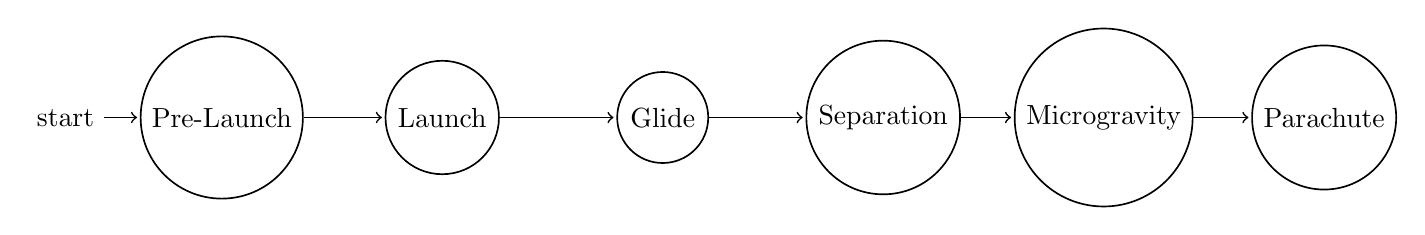
\begin{tikzpicture}[->,shorten >=1pt,auto,node distance=2.8cm,semithick]
  \node[initial,state]	(P)			{Pre-Launch};
  \node[state]	(L) [right of=P]	{Launch};
  \node[state]	(G)	[right of=L]	{Glide};
  \node[state]	(S)	[right of=G]	{Separation};
  \node[state]	(M)	[right of=S]	{Microgravity};
  \node[state]	(C)	[right of=M]	{Parachute};
  \path	(P)	edge [right]	node{}	(L);
  \path	(L)	edge [right]	node{}	(G);
  \path	(G)	edge [right]	node{}	(S);
  \path	(S)	edge [right]	node{}	(M);
  \path	(M)	edge [right]	node{}	(C);
  \end{tikzpicture}
  \caption{Conceptual state diagram for payload avionics.}
\end{figure}

For example, during the pre-launch state we can effectively ignore all sensor readings until we see a very high acceleration on the z axis, which signals launch.  We can begin logging all sensor values from that point on (or even retroactively record a set of rolling pre-launch values) until we see the z axis acceleration end, which signals that we have entered the glide state.  Obviously we will need to look at more than a single sensor value to transition between states, but the general idea is to understand what we can expect during each phase of launch, and encode those conditions as state transitions.

The major design concern for payload avionics are that accuracy is more important than precision.  A false early start would risk damaging or completely destroying the rocket with the payload propellers, but a late start would only risk missing some or all of the experimental data.

\subsubsection{Avionics Testing}
The CS and ECE teams will be writing avionics for the rocket and payload which will be able to determine when separation should occur. Due to the high degree of precision that this requires and the significant negative consequences of failure for this code, ensuring the functionality of this code is of the utmost importance. It is also standard within the aerospace industry to very thoroughly test any and all avionics code.  Writing a thorough test suite will be good practice for working within the aerospace or related industries. There are three types of testing that the team has decided to carry out: hardware tests, unit tests, and simulations with randomization. The CS team will cooperate with the ECE team to perform hardware tests.

Hardware tests will involve making certain that each sensor is functional, powered, and giving reasonable readings.  Joshua will take responsibility to ensure that every electronic component on both the payload and the rocket have been thoroughly tested.

Unit tests will involve making sure that the basic functionality of the code is intact. This will mean ensuring that the programs and functions written to read from sensors give accurate output to a given input. These will mostly be used to test code reading from sensors, or that the code will trigger certain events when given input that should do so. Some tests may be written to ensure a minimum degree of robustness, such as throwing out inputs that are invalid (such as an input that is a string of characters that should be a number). Joshua will oversee the writing of unit tests on avionics code. He will check to ensure that the goals for line coverage are met by the unit tests, and aim to have the unit tests ensure all code functions correctly to expected inputs.

The final aspect of testing the avionics code is to simulate a launch with robustness testing. This will involve encapsulating the functionality of the code for triggering flight events in some manner, and then testing that code against simulated inputs. These inputs will then be randomly altered in a variety of manners. If possible, this will be extended to include testing of code for sensor interaction, with the code interacting with simulated sensors rather than actual sensors. The randomization will likely take one of the following forms, but may include other forms if the code calls for it.

\begin{itemize}
\item Throwing a value that is out of bounds (this included the following)
\begin{itemize}
\item A value that is of the wrong type
\item A value that is too large
\item A value that is too small
\end{itemize}
\item Having a sensor cease responding
\item Having a sensor continually send the same value
\item Offsetting a sensor’s outputs by some set amount for the rest of the launch
\item Having a sensor feed a value that is not out of bounds, but is not correct
\item Having a sensor feed values for the rest of the launch that are incorrect and
\begin{itemize}
\item in bounds 
\item out of bounds
\item either in or out of bounds
\end{itemize}
\end{itemize}

The number of randomized failures will be able to be set at the start of the test, but not timing or the types of failures. Some failures may be weighted as being more significant, and therefore valued as a larger number of failures. The test will not be given a clear pass fail, but will instead push the outputs of the avionics code to a csv, which will be compared against the csv output of the code with no randomization as well as the inputs given by the simulation.

\subsection{Telemetry and Parsing Flight Data}

\subsubsection{Transmitting Telemetry}

The ECE subteam selected the BigRedBee BeeLineGPS telemetry module which cannot be used with additional sensors and only transmits using APRS formatting.  This means that we cannot control which fields are being transmitted, or the packet formatting of the telemetry data.  Each transmitter will send a packet once per second, containing the latitude, longitude, and altitude of the transmitter.  These packets will be transmitted as audio data and can be decoded into a string in the APRS format.

There will be two telemetry transmitters in use during the flight.  One will be in the nosecone of the rocket, and the other will separate with the payload.  They will be on slightly different radio frequencies because the timing is not guaranteed, so the signals may overlap.

\subsubsection{Receiving Telemetry}
\label{subsec:telemetry}

Levi Willmeth will manage receiving telemetry and parsing flight data for this project.

We will be using a software TNC called Direwolf to decode the audio tones into strings of text.  Because the timing is not guaranteed and the signals may overlap, we will be using one primary receiver per radio signal, with an additional secondary receiver for redundancy.  We expect to use four raspberry pi zeros to receive two incoming radio signals, to provide redundancy during signal processing.

\begin{center}
	\includegraphics[width=0.65\textwidth]{images/parser_diagram.eps}
    \label{flow-of-data}
    \captionof{figure}{Flow of information into the parser.}
\end{center}

% Processing each signal will be done using affordable Raspberry Pi Zero computers, which will be connected and networked to a more powerful Raspberry Pi 3 B computer, using an OTG USB cable.  This will allow each of the parsing computers to be powered and networked using a single wire.  All of the ground computers will be housed in a portable, hard-shell carrying case that also contains a USB power bank.  This will allow us to turn on the system, and begin parsing on multiple radio channels without any additional steps.

When the parsing computers boot up, they will immediately begin running the Direwolf software that allows them to receive an audio source and parse it into a string of text.\cite{direwolf}  They will also begin running a Python script to take the input string from Direwolf, validate it for content, and insert individual fields into a database on the local network.  The database will be described in section \ref{subsec:database} of this document.  These programs will be started as services so that they can be stopped, started, or automatically restart themselves as needed.\cite{script-as-service}\\

\begin{lstlisting}[frame=single]
2017-11-28 14:15:56UTC,ESRA-1,131812h3521.00N/07820.00W,496650,8642,446.875,PL
\end{lstlisting}
\label{example-aprs}
\captionof{figure}{Example APRS packet.}

Each incoming radio packet may be from our rocket, or it may be from an unrelated transmitter on the same frequency.  This is because we are using uncontrolled analog radio frequencies that may contain information from other, unknown users.  We will use Python to parse the string, validate that it contains the correct radio call sign for our payload or rocket, and perform a checksum to test for corruption during transmittal.

If the packet does not pass checksum, contains an invalid call sign, or does not contain the correct data fields, a warning will be added to the parser log and the string will be inserted into a special database table for invalid inputs.  This will allow us to inspect errors without discarding any data.

\subsubsection{Parsing Data}

The parsing program described in \ref{subsec:telemetry} will be configured to either process incoming strings from Direwolf, or to accept a well formatted file.  This will allow the same parsing program that listens for radio inputs to parse the data recorded and stored on board the rocket and payload during flight.

After the flight, a human operator will be able to remove the SD card from the rocket and payload avionics flight computers, plug the SD card into a laptop, and point the parsing program at the SD card.  Using the appropriate table name and steps similar to those used while parsing radio inputs, the import program will split the strings into individual fields and insert them into the database over the network.\\

\begin{lstlisting}[frame=single]
timestamp,acc_x1,acc_x2,acc_x3,acc_y1,acc_y2,acc_y3
2017-11-28 14:15:56UTC,27.2,56.7,32.2,234.2,235.7,463.4
2017-11-28 14:15:57UTC,27.1,56.7,32.2,234.2,235.7,463.4
2017-11-28 14:15:58UTC,27.2,56.8,32.2,234.2,235.7,463.4
\end{lstlisting}
\label{example-file}
\captionof{figure}{Example avionics output file.}


\subsection{Database}
\label{subsec:database}

Levi Willmeth will set up and manage a MariaDB database for this project.

This project will collect several hundred thousand lines of sensor data, using several different sources.  All of this data will need to be sortable and searchable in order to interpret the results of our flight.  Furthermore, we want to be able to record and analyze different flights independently.  Using a database to store our flight data will allow us to accomplish all of these goals.

Because the rocket avionics records different types of sensors than the payload avionics or the radio telemetry modules, we will use one table per type of data source.  That means one table will hold all data received from a BeeLineGPS telemetry module, another table will hold all data imported from the payload avionics, and so on.  These tables will also need to relate to each other in order to allow the display program to make appropriate connections between different sensors recorded on different hardware.  This will be done using a Flight table with a primary key that will be used as a foreign key on each of the individual data tables.

\begin{center}
	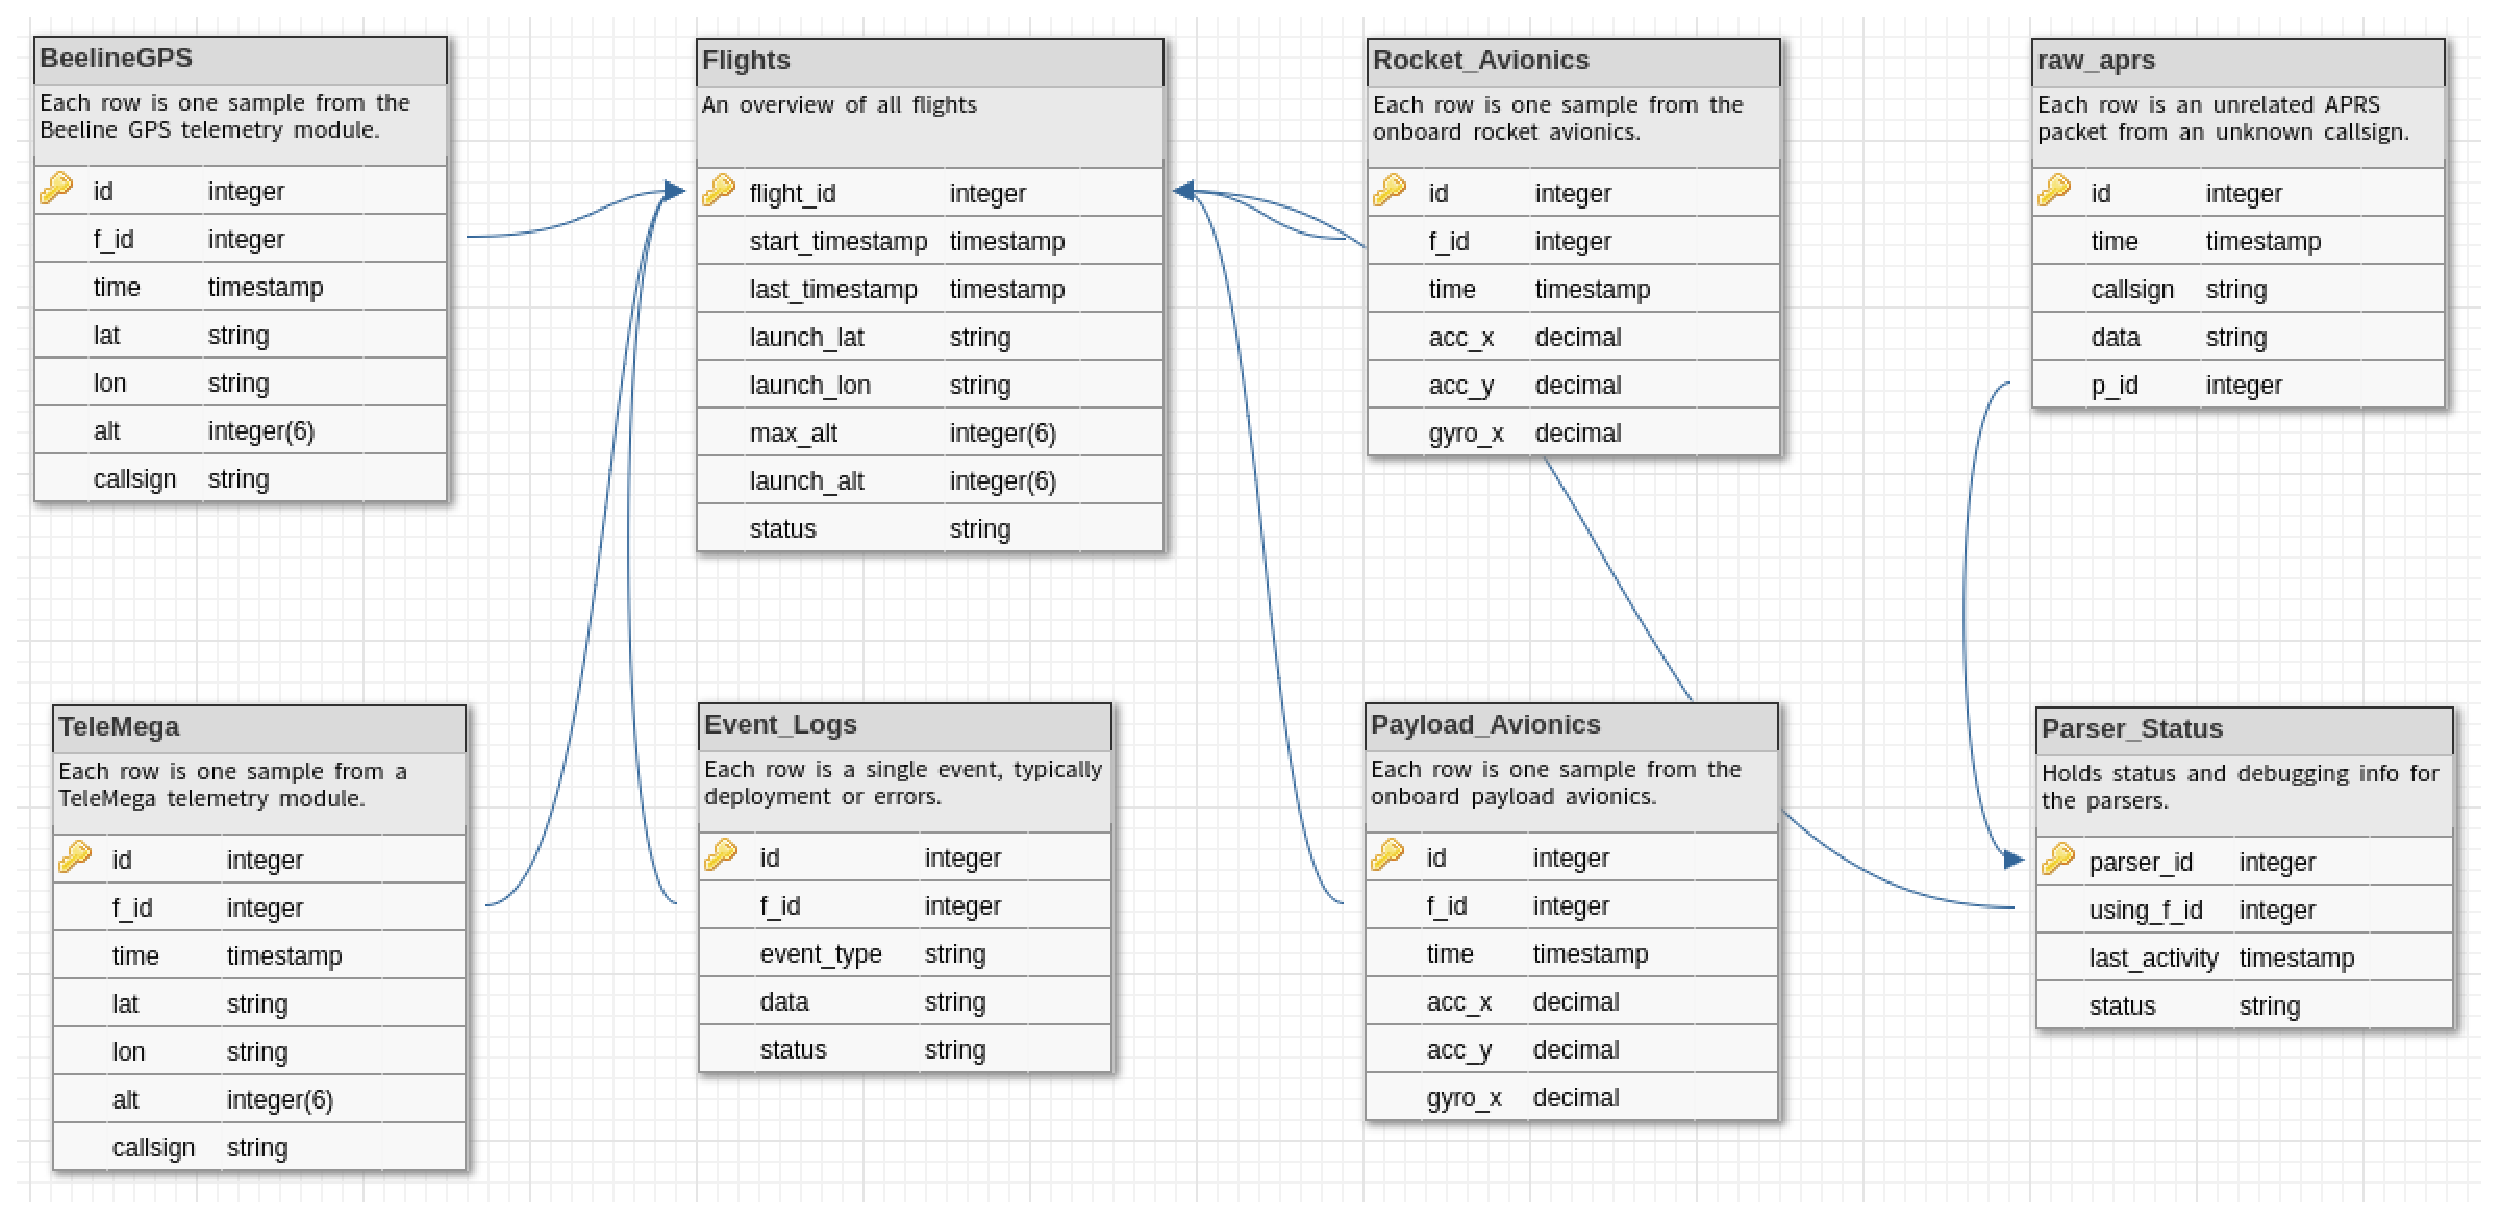
\includegraphics[width=\textwidth]{images/database_schema_v102.eps}
    \label{database-schema}
    \captionof{figure}{Early draft of the database schema.}
\end{center}

When the telemetry parsing Python script begins, it will check the Flights table of the database to see if there is a flight record with an Active status.  This table and field will be used to synchronize the parsers so that records from one radio frequency can be related to records from another frequency at the same time.  The Flights table has a primary key called 'flight\_id' that is used as a foreign key on other related tables.

To eliminate duplicate rows caused by using redundant receivers, we will use a MySQL query that first checks if a row exists, before inserting a new row.  This can be done as a single query: \cite{unique-sql-insert}

\begin{lstlisting}[frame=single]
INSERT INTO
	BeelineGPS (f_id, time, lat, lon, alt, callsign)
SELECT
	* FROM (SELECT $cur_time, $cur_flight_id) AS tmp
WHERE NOT EXISTS (
    SELECT id FROM BeelineGPS WHERE time = $cur_time
) LIMIT 1;
\end{lstlisting}

There may be situations where a given timestamp contains data across multiple tables.  For example, the rocket avionics may record some types of data at 100 Hz, and other types of data at only 10 Hz.  Some of these records may share an identical timestamp, others may not.  That is why we are using multiple tables and a foreign key instead of one larger table and assuming our timestamp is unique.

While graphing this data, we are likely to want to relate data from different tables.  For example if we recorded latitude and longitude in the BeelineGPS table, and acceleration in the Rocket\_Avionics table, we may want to combine that data to see our acceleration at different points across a map.  This is where the database becomes exceptionally useful compared to flat files.  We can use a join query to select records from both tables, based on the knowledge that they will have identical f\_id's and similar timestamps.  The syntax would look something like this:

\begin{lstlisting}[frame=single]
SELECT
	BeelineGPS.lat, BeelineGPS.lon, Rocket_Avionics.acc_x
FROM
	BeelineGPS
INNER JOIN
	Rocket_Avionics
ON
	BeelineGPS.f_id=Rocket_Avionics.f_id
WHERE
	BeelineGPS.flight_id=$cur_flight;
\end{lstlisting}

In this example the latitude may be sampled at only 1 Hz while acceleration could be sampled at closer to 100 Hz.  We could choose to average out many acceleration values to find the best fit at the moment we recorded the latitude, or we could let MySQL find a single value using the Rocket\_Avionics timestamp closest to the BeelineGPS timestamp.

\subsection{Display Components}

\subsection{Networking}
Allison will set up networking between the ground station Raspberry Pis.

The ground station will consist of a Raspberry Pi 3, several radio receivers, several Raspberry Pi Zeros, and a battery. 
The Raspberry Pi zeros will parse data received through the radios before sending it to the database and server hosted on the Raspberry  Pi 3. 
The server will allow users to connect through an ad hoc network and display the graphical flight data on mobile devices. 

USB OTG (On-The-Go) will be used to connect the four Pi Zeros to the Pi 3B, which can then assign them IP addresses and power the other Pis. 
Setting up this connection is a relatively straightforward process that involves editing configuration files on the zeros to give them static IP addresses, and configuring the host Pi to forward network information and assign static IP addresses to each wired connection. \cite{OTG}

The connected Pis will also serve the graphed flight data to mobile devices around the ground station.
This will be accomplished through an ad hoc network. 
The Pi 3B has an integrated wifi module and changing the interface configuration file at /etc/network/interfaces will allow the the Pi to operate in ad hoc mode. \cite{config-adhoc}

\subsubsection{Web hosting}

Allison will manage the web-based user interface for graph viewing.

The dynamic graphing display will be hosted by an Node.js server running on a networked Raspberry Pi 3B. 
Using express-handlebars, we will be able to display many different graphs while reusing code through partials. 
The flight data graphs generated by the dynamic graphing program will be served as HTML pages to connected mobile devices.
Users will be able to select flights and graph types to view on their personal devices while connected to the network.


\subsubsection{Dynamic graphing}

Dynamic Graphing will be managed by Joshua Novak.

The dynamic graphs will be written in JavaScript, using the non-commercial version of CanvasJS. The graphs will be able to be displayed in an HTML page, and will update through queries to a database. These updates will be once a second, though new data may not be displayed if it is not available.

At least the following charts will be displayed in the form of dynamic graphs
\begin{itemize}
\item Location of the rocket on a map
\item Altitude of the rocket
\item Vertical velocity of the rocket
\end{itemize}

The following will be analyzed for launches
\begin{itemize}
\item Temperature
\item Velocity
\item Acceleration
\item Barometric pressure
\end{itemize}

The first kind of graph that will be displayed is the map. The map will be generated with basic JavaScript. An image of a map around the launch site will be used, with javascript overlaying dots representing the recorded locations of the rocket. The dots will have an on hover effect to display the GPS coordinates of that point, and the timestamp associated with it. Some additional effects may be added to make the graph more readable, such as gradually changing the hue of dots over time, so that newer points appear different from older ones. This will only be used to show the location of the rocket on a map. The points at which particular flight events occur may be represented with a different image, such as a broken circle for separation, or a half circle once the parachute is deployed.

The other kind of graph that will be used is a basic value vs time graph. This graph will likely be generated using CanvasJS. It will display a maximum number of points relative to the size of the window, so that the graph scales well to different display sizes. These points will be the last several datapoints for the flight. The time will be determined by the timestamp. The relevant value to be graphed opposing time will generally be taken directly from the database query where it is available, and calculated from other data when it is not available but can be calculated with a reasonable degree of accuracy. This will likely be used for all other fields.

Finally, we will use R for analyzing data recovered from the Payload and the Rocket. This will be better suited for the task, as we want to be able to find and ignore outlier data as well as generate lines of best fit.
% ==============================================================================

\bibliography{references}
\bibliographystyle{IEEEtran}
\end{document}
